%%%%%%%%%%%%%%%%%%%%%%%%%%%%%%%%
% Chap 4. Experiments
%%%%%%%%%%%%%%%%%%%%%%%%%%%%%%%%

\chapter{Experiments}\label{chapter4}

\section{Setup} \label{chap4:sec:setup}

For our experiments, we use the OpenAI Safety Gym \cite{PPO-Lagrangian, Safety-Gymnasium} environments.
OpenAI no longer maintains Safety Gym, and its development has been continued since 2023 by the PKU-Alignment Team under the name Safety Gymnasium.
Safety Gymnasium preserves full compatibility with the original Safety Gym environments, including identical reward functions, cost functions, agents, and other components.
To avoid confusion, we refer to these environments as Safety Gym throughout this thesis.
In Safety Gym environements, there are three types of agents: Point, Car, and Doggo.
In our experiments, we use the Car agent provided in Safety Gym.
\begin{itemize}
    % \item \textbf{Point}: A simple 2D robot with two actuators—one for turning and another for forward/backward motion. The Point agent appears on the far left in Fig.~\ref{chap4:fig:cost}.
    \item \textbf{Car}: A car-like robot with two independently controlled front wheels and a passive rear wheel. Since both forward movement and turning must be controlled together, it is slightly more difficult to operate than the Point. The Car agent is shown in Fig.~\ref{chap4:fig:reward}.
\end{itemize}
Also, there are three types of tasks: Goal, Button, and Push.
We use two of the tasks provided in Safety Gym: Goal and Button.
\begin{itemize}
    \item \textbf{Goal}: The agent must reach a goal location while avoiding obstacles.
    \item \textbf{Button}: The agent must press a button while avoiding obstacles.
    \item \textbf{Push}: The agent must push yellow box to a goal location while avoiding obstacles.
\end{itemize}
The reward function provides positive rewards as the agent moves closer to the goal, and negative rewards as it moves farther away:
$ r_t = d_{t - 1} - d_t $, where $d_t$ is the distance to the goal at time $t$.
Additionally, each task provides an extra positive reward when the agent successfully completes the objective, such as reaching the goal, pressing a button, or moving a box.
\begin{figure*}[h]
  \centering
  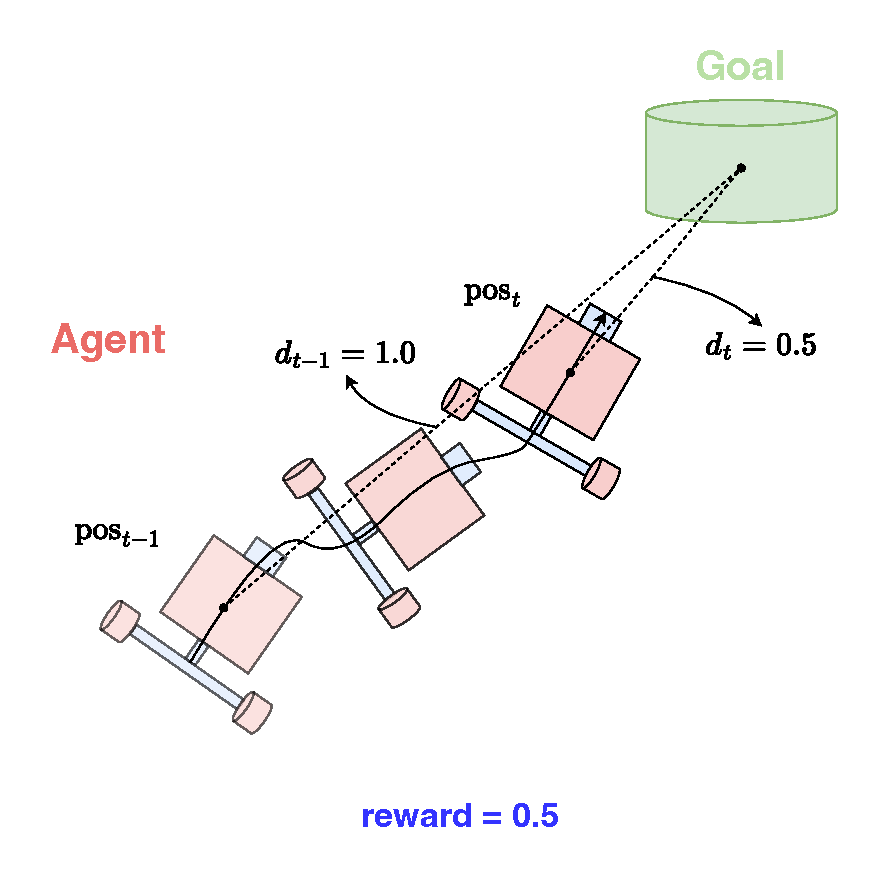
\includegraphics[width=0.5\textwidth]{imgs/chap4/setup/reward.pdf}
  \caption{Illustration of how reward is computed in the Safety Gym}
  \label{chap4:fig:reward}
\end{figure*}

\begin{figure*}[h]
  \centering
  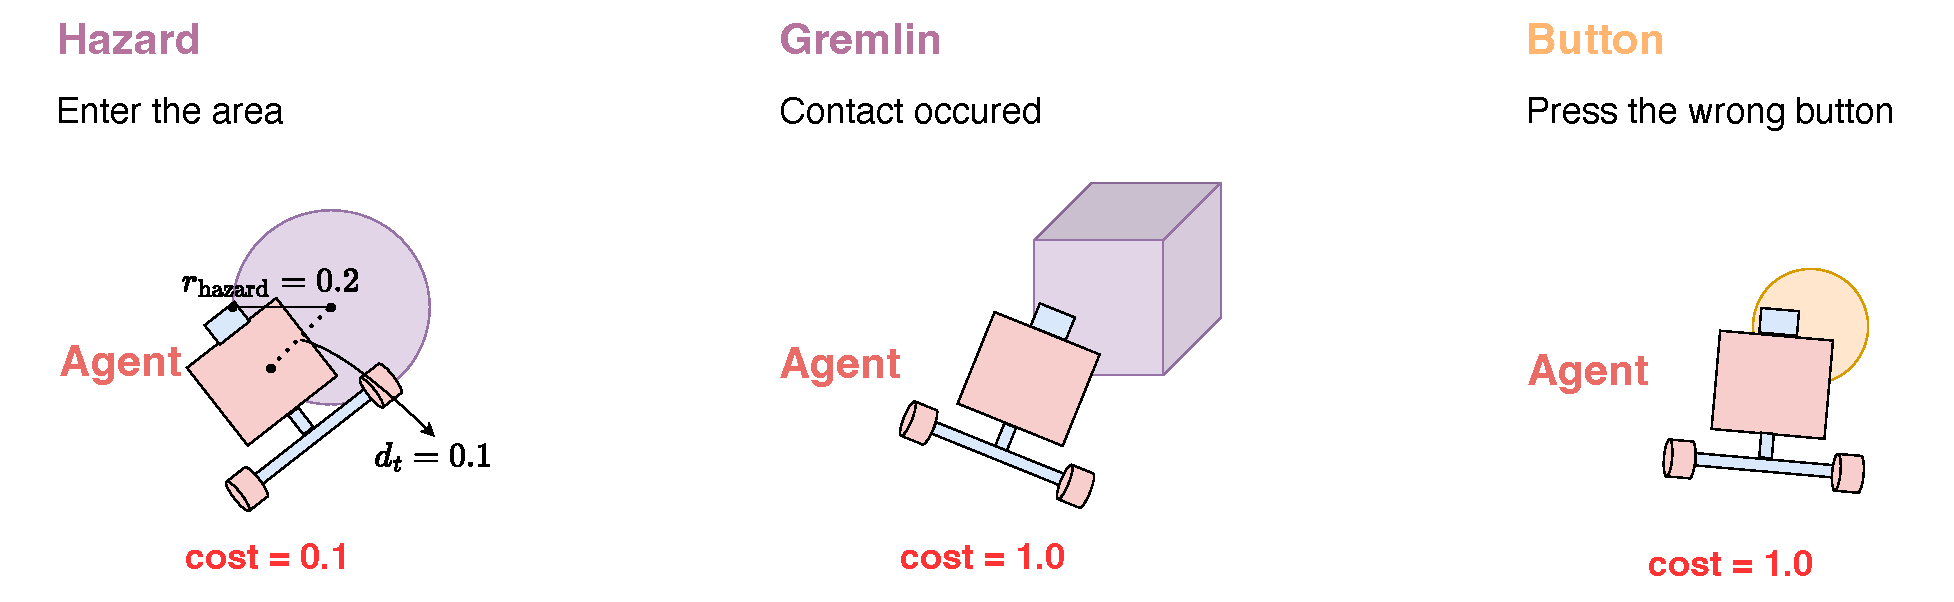
\includegraphics[width=1.0\textwidth]{imgs/chap4/setup/cost.pdf}
  \caption{Illustration of how costs are computed in the Safety Gym}
  \label{chap4:fig:cost}
\end{figure*}

The cost function varies depending on the types of obstacles present in each task.
In our experimental environments, three types of obstacles are used, as illustrated in Fig.~\ref{chap4:fig:cost}:
\begin{itemize}
    \item \textbf{Hazard}: A cost is assigned when the agent enters a hazard area. The cost is computed as $c_t = d_t - r_{\text{hazard}}$, where $d_t$ is the distance from the agent to the center of the hazard and $r_{\text{hazard}} = 0.2$ is the hazard radius.
    \item \textbf{Gremlin}: A cost of $-1.0$ is incurred when the agent makes contact with the gremlin object.
    \item \textbf{Button}: A cost of $-1.0$ is assigned when the agent presses a button that is not the designated goal button.
\end{itemize}
A key distinction of this thesis compared to other works lies in how the cost function is defined.
Safety Gym provides two options for computing cost: a dense formulation and a sparse (indicator) cost.
Many prior works adopt the sparse cost, where the environment returns 1 if a cost-triggering event occurs and 0 otherwise.
In contrast, this thesis uses the dense cost described above, where the cost value is computed at each time step based on factors such as distance to obstacles or safety-related conditions.
This choice is motivated by the fact that using sparse costs makes it difficult to precisely define and enforce constraint conditions.
Dense costs allow for more precise and informative constraint definitions compared to sparse costs.

%%%%%%%%%%%%%%%%%%%%%%%%%%%%%%%%
\section{Analyzing the Influence of alpha in the Feasible Actor-Critic} \label{chap4:sec:experiments:fac}
%%%%%%%%%%%%%%%%%%%%%%%%%%%%%%%%

As discussed in Section~\ref{chap2:sec3:sac}, Soft Actor-Critic (SAC) promotes stochastic exploration by maximizing both expected return and policy entropy. 
The temperature parameter $\alpha$ controls the importance of the entropy term: larger values of $\alpha$ encourage more exploratory and diverse action selection.
However, in the Feasible Actor-Critic (FAC) framework, this exploration objective can conflict with the effect of the Lagrange multiplier, which encourages the policy to satisfy safety constraints.
To examine this trade-off, we compare the training performance of unconstrained SAC (yellow curve) and FAC with various fixed $\alpha$ values, using Fig.~\ref{chap4:fig:fac_return}, Fig.~\ref{chap4:fig:fac_cost}.
In Figure~\ref{chap4:fig:fac_cost}, although small spikes are present, FAC with all tested $\alpha$ values generally maintains a lower cost compared to unconstrained SAC.
This indicates that the constraint-satisfying mechanism in FAC is working as designed, leading to lower cost return by enforcing state-wise constraints more effectively.
On the other hand, the return curves in Figure~\ref{chap4:fig:fac_return} reveal that with $\alpha = 0.001$ (green), the return improves rapidly in the early phase (up to around 200 epochs), but then gradually declines and converges toward zero.
This behavior suggests that when $\alpha$ is relatively large, the entropy term dominates the learning signal, making the policy overly stochastic and less sensitive to both reward and constraint signals—ultimately degrading policy performance.
Based on these observations, we fix $\alpha$ to a small value of $0.00001$ for all subsequent comparisons between FAC and our proposed method, to minimize the entropy-induced instability while retaining some degree of exploration.

\begin{figure*}[h]
  \centering
  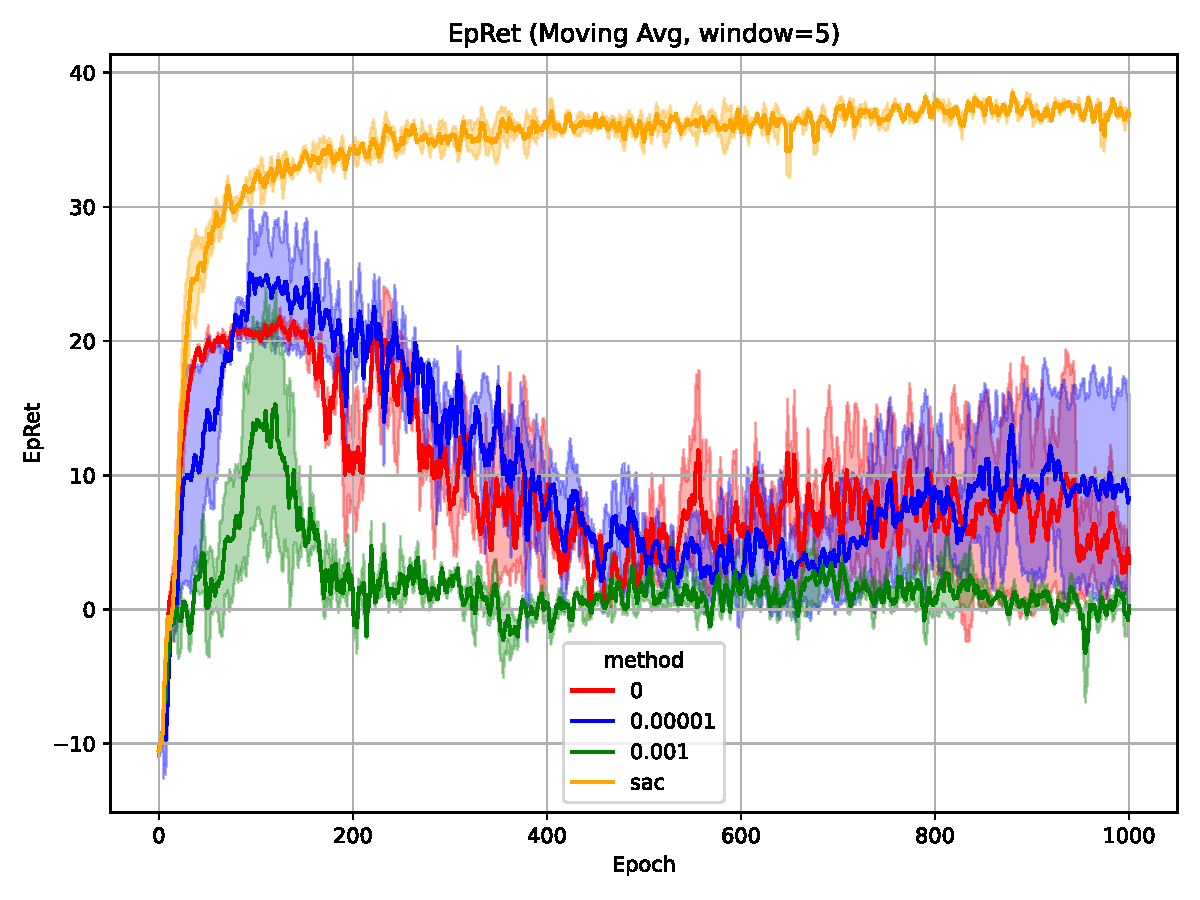
\includegraphics[width=0.65\textwidth]{imgs/chap4/fac/return.pdf}
  \caption{Training curves of return over epochs for different temperature parameters $\alpha$ in the Feasible Actor-Critic algorithm}
  \label{chap4:fig:fac_return}
\end{figure*}

\begin{figure*}[h]
  \centering
  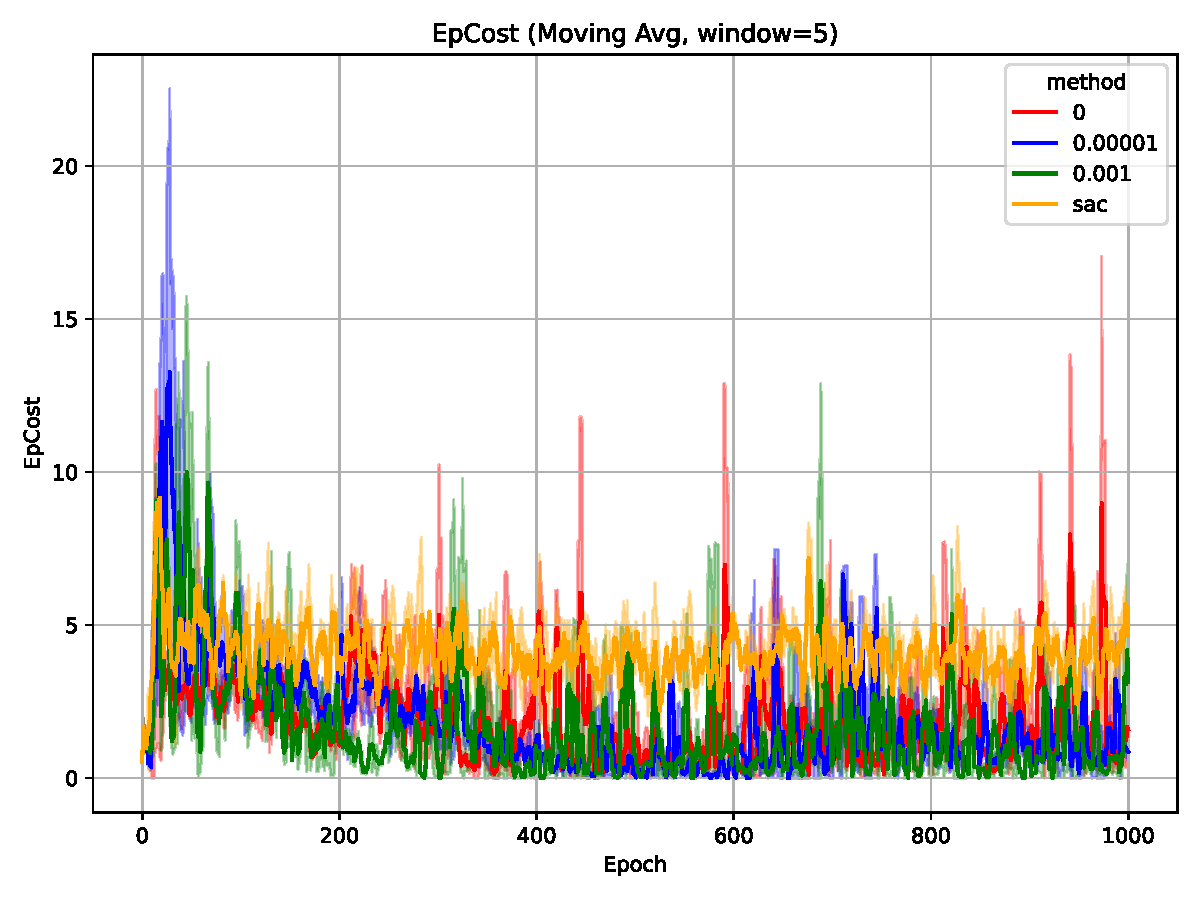
\includegraphics[width=0.65\textwidth]{imgs/chap4/fac/cost.pdf}
  \caption{Training curves of cost return over epochs for different temperature parameters $\alpha$ in the Feasible Actor-Critic algorithm}
  \label{chap4:fig:fac_cost}
\end{figure*}

\clearpage

\begin{table}[h]
  \centering
  \caption{Hyperparameters used in Experiment \ref{chap4:sec:experiments:fac}}
  \label{tab:hyperparams-fac}
  \begin{tabular}{l c}
    \toprule
    \textbf{Hyperparameter} & \textbf{Value} \\
    \midrule
    Environment                         & Car Goal \\
    Number of epochs                    & 1000 \\
    Number of steps per epoch           & 2000 \\
    Batch size                          & 256 \\
    Hidden layer size (MLP)             & 256 \\
    gamma (discount factor)             & 0.99 \\
    polyak (target network update)      & 0.995 \\
    Learning rate (policy)              & 5e-6 \\
    Learning rate (value function)      & 1e-3 \\
    Learning rate (Lagrange multiplier) & 5e-8 \\
    Lagrange multiplier init (bias)     & 0 \\    
    \bottomrule
  \end{tabular}
\end{table}

%%%%%%%%%%%%%%%%%%%%%%%%%%%%%%%%
\section{Analyzing the Influence of Bias Initialization in the Lagrange Multiplier Network of PPO Lagrangian Network} \label{chap4:sec:experiments:lagrange_init}
%%%%%%%%%%%%%%%%%%%%%%%%%%%%%%%%

Lagrangian-based methods are known to be sensitive to both initialization and learning rate \cite{CRL-survey}. 
Improper initialization of the Lagrange multiplier network can lead to suboptimal or delayed policy convergence. 
In particular, a large initial value may overly penalize the policy, driving it prematurely toward a local optimum, while a small initial value may result in slow adaptation of the constraint enforcement.
To analyze the effect of bias initialization,  we conducted experiments by varying the initial bias value of the final layer in the Lagrange multiplier network. 
Specifically, we manually initialized the bias term of the last linear layer to one of four values: 0, 20, 40, and 60.

\begin{figure*}[h]
  \centering
  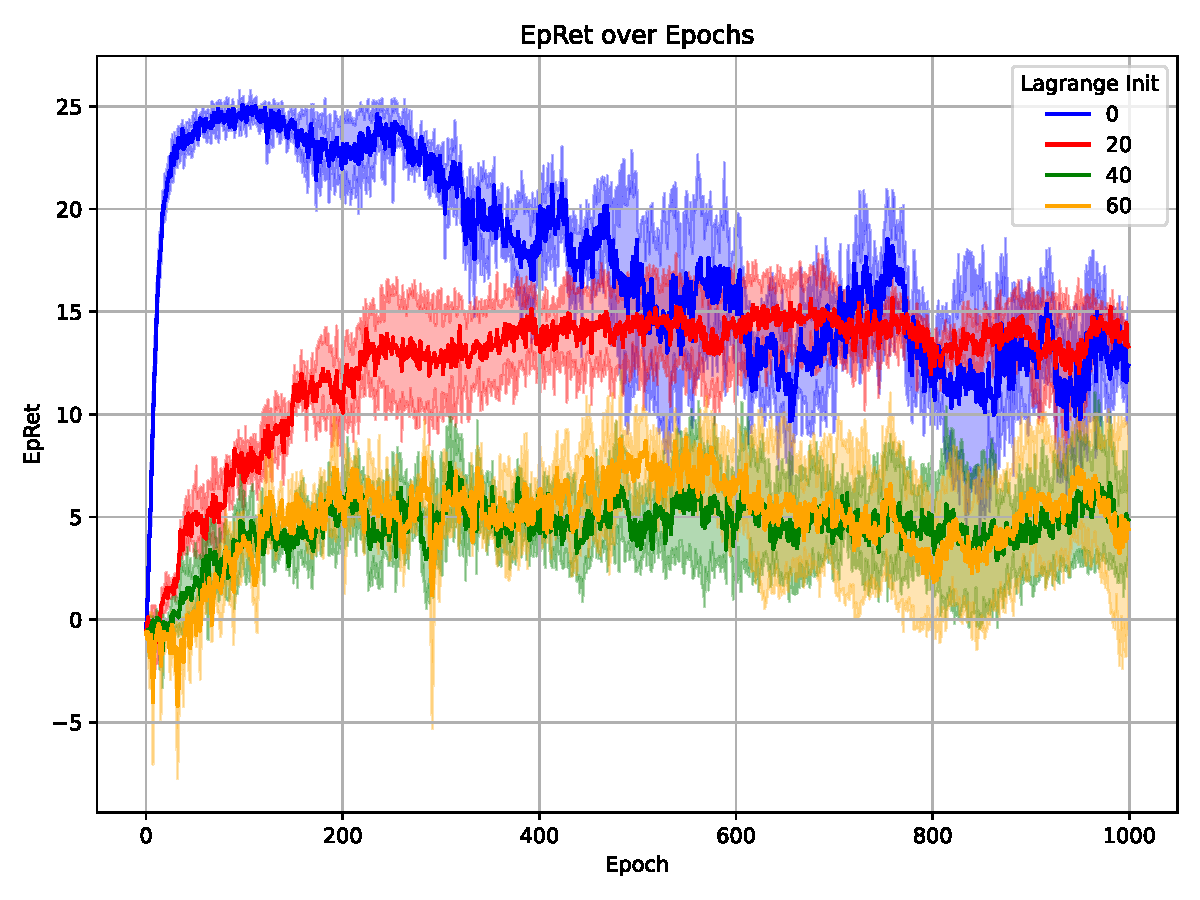
\includegraphics[width=0.65\textwidth]{imgs/chap4/lagrange_init/return.pdf}
  \caption{Training curves of return over epochs for different bias initializations in the Lagrange multiplier network}
  \label{chap4:fig:lagrange_init_return}
\end{figure*}

In Fig.~\ref{chap4:fig:lagrange_init_return}, shows the training curves of return over 1000 epochs for different bias initializations of the Lagrange multiplier network.
Although the convergence behavior varies across initial values, all four settings demonstrate stable policy learning overall.
When the initial bias is set to 0, the early phase (epoch $0 \sim 300$) closely resembles unconstrained PPO, showing a rapid increase in return.
However, as the Lagrange multiplier values grow, the return gradually decreases, indicating stronger constraint enforcement over time.
With an initial bias of 20, the agent achieves the most stable and effective learning performance, maintaining high return while satisfying constraints.
In contrast, higher initializations (40 and 60) result in excessive penalty signals, which overly constrain the policy.
This leads to premature convergence to suboptimal solutions, likely due to limited exploration or overly conservative policy updates.

\begin{figure*}[h]
  \centering
  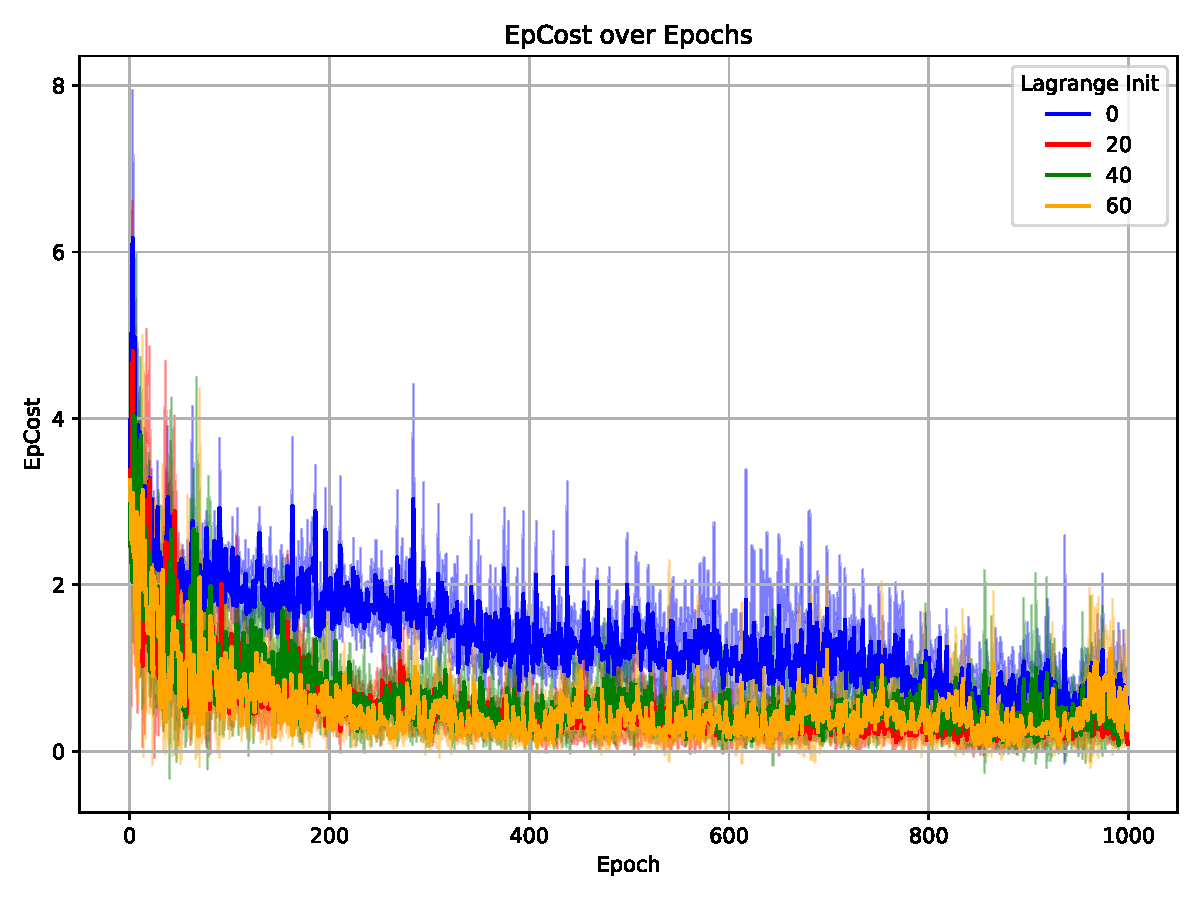
\includegraphics[width=0.65\textwidth]{imgs/chap4/lagrange_init/cost.pdf}
  \caption{Training curves of cost return over epochs for different bias initializations in the Lagrange multiplier network}
  \label{chap4:fig:lagrange_init_cost}
\end{figure*}

As shown in Fig.~\ref{chap4:fig:lagrange_init_cost}, all four settings demonstrate a stable reduction in cost over the course of training.
This indicates that the Lagrange multiplier network, regardless of initialization, is able to learn to enforce constraints effectively.
However, when comparing the results more closely, we observe that the setting with an initial bias of 0 achieves less cost reduction compared to the setting with an initial bias of 20, despite both eventually reaching similar Lagrange multiplier values (see Fig.~\ref{chap4:fig:lagrange_init_lagrange}). 
This suggests that early enforcement of constraints plays an important role in guiding the policy to safer regions of the state space.
In the zero-initialization case, the Lagrange multiplier grows more slowly, allowing higher constraint violations in the early phase of training.
As a result, the policy may have already been shaped in a way that is less sensitive to cost signals, making later enforcement of constraints less effective and leading to suboptimal cost minimization.
Therefore, initializing the Lagrange multiplier with a moderately large value (e.g., 20) helps stabilize training by better balancing the trade-off between reward and cost throughout learning.

\begin{figure*}[h]
  \centering
  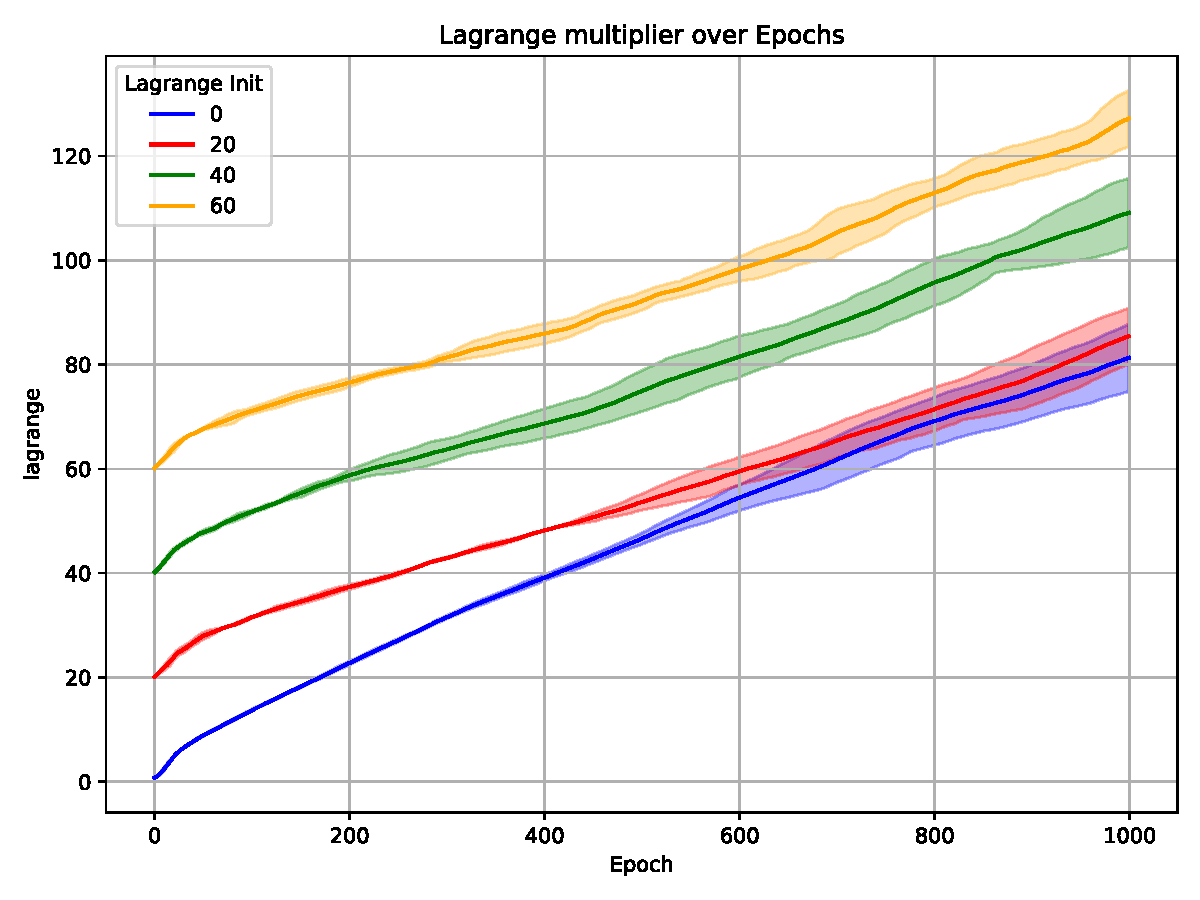
\includegraphics[width=0.65\textwidth]{imgs/chap4/lagrange_init/lagrange.pdf}
  \caption{Training curves of Lagragne multiplier over epochs for different bias initializations in the Lagrange multiplier network}
  \label{chap4:fig:lagrange_init_lagrange}
\end{figure*}

%%%%%%%%%%%%%%%%%%%%%%%%%%%%%%%%
\section{Analyzing the Influence of Learning Rate in the Lagrange Multiplier Network of PPO Lagrangian Network} \label{chap4:sec:experiments:lagrange_lr}
%%%%%%%%%%%%%%%%%%%%%%%%%%%%%%%%

The learning rate of the Lagrange multiplier network also plays a crucial role in stability and convergence. 
If the learning rate is too high, the multiplier may oscillate excessively, causing unstable policy updates. 
Conversely, if it’s too low, the multiplier may adapt too slowly to apply appropriate penalties.
To analyze the effect of the learning rate in the Lagrange multiplier network, we conducted experiments by varying the learning rate used for optimizing the network parameters.
Specifically, we tested three different learning rate values: 0.0003, 0.003, and 0.03.

\begin{figure*}[h]
  \centering
  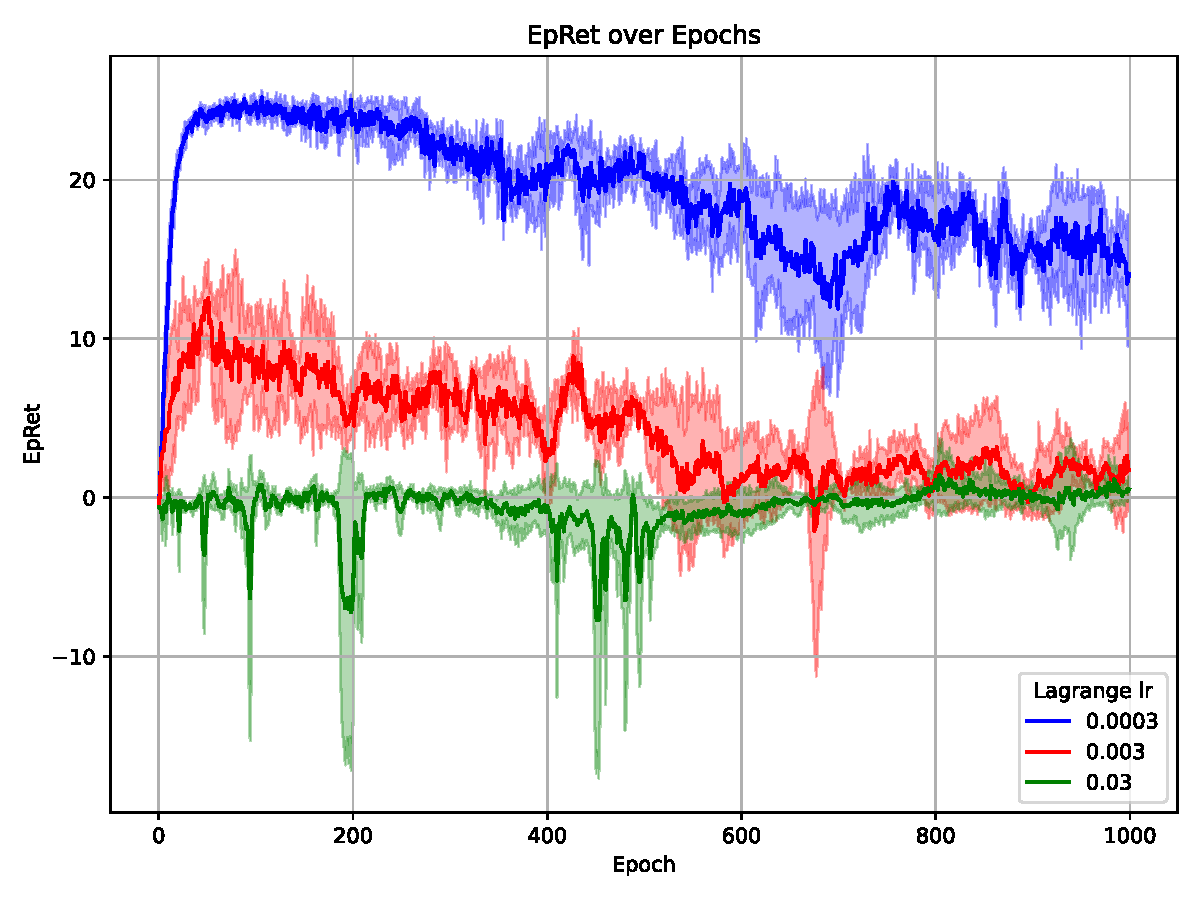
\includegraphics[width=0.65\textwidth]{imgs/chap4/lagrange_lr/return.pdf}
  \caption{Training curves of return over epochs for different learning rate initializations in the Lagrange multiplier network}
  \label{chap4:fig:lagrange_lr_return}
\end{figure*}

\begin{figure*}[h]
  \centering
  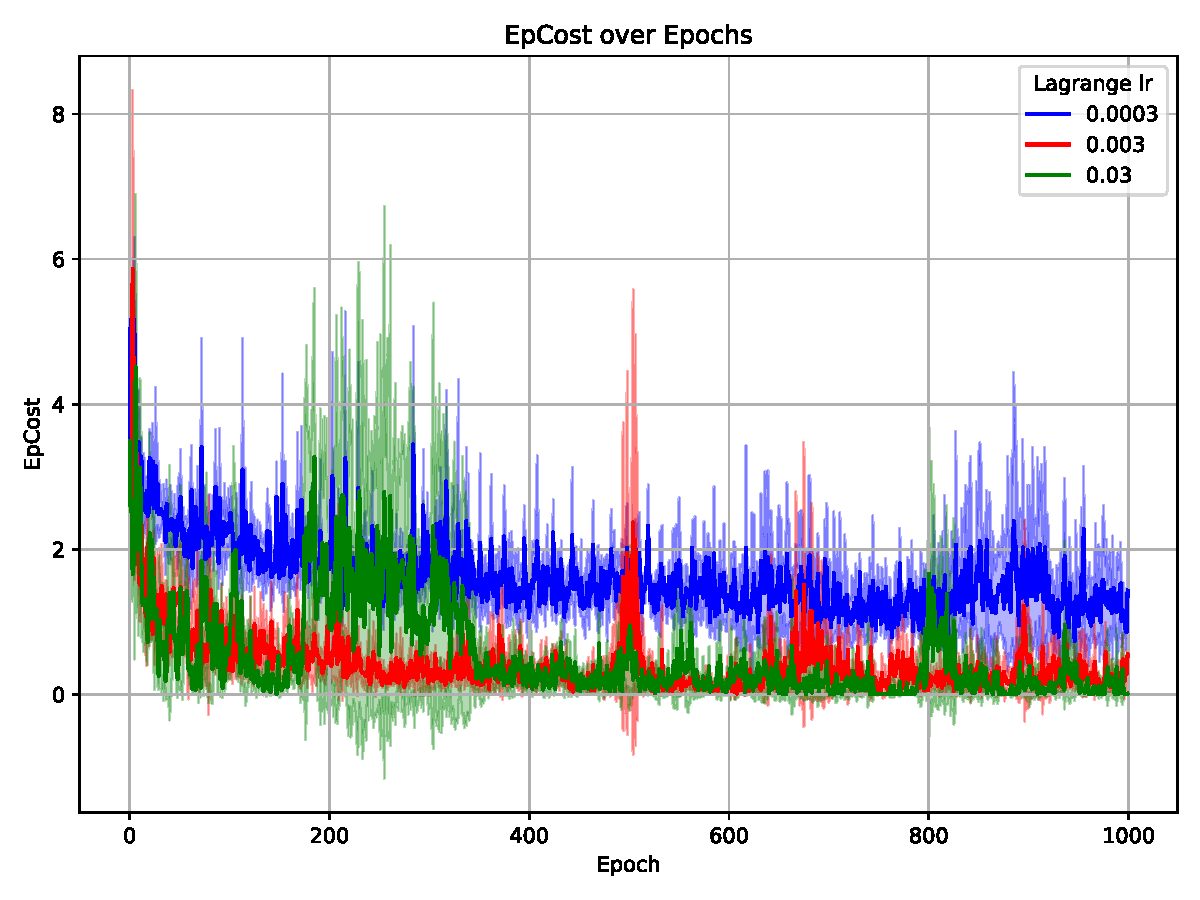
\includegraphics[width=0.65\textwidth]{imgs/chap4/lagrange_lr/cost.pdf}
  \caption{Training curves of cost return over epochs for different learning rate initializations in the Lagrange multiplier network}
  \label{chap4:fig:lagrange_lr_cost}
\end{figure*}

\begin{figure*}[h]
  \centering
  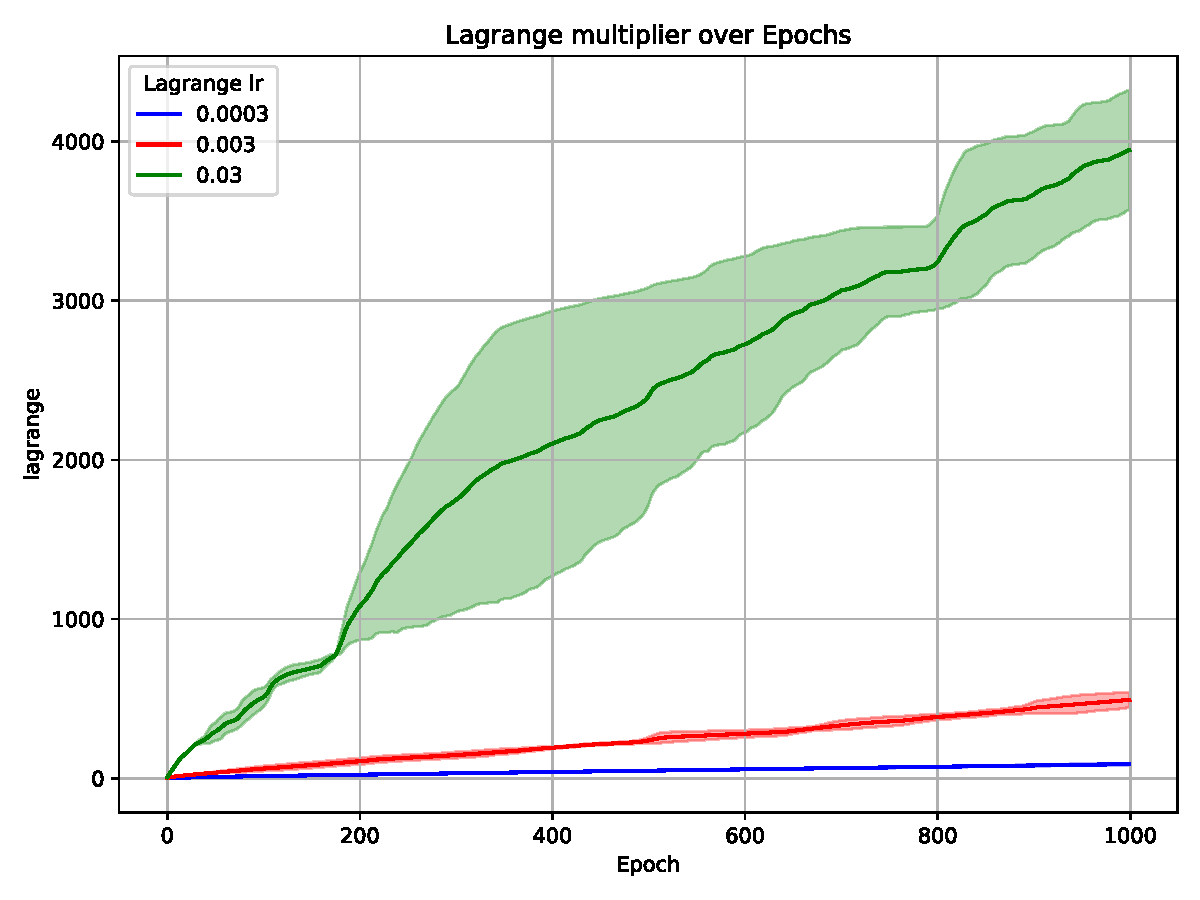
\includegraphics[width=0.65\textwidth]{imgs/chap4/lagrange_lr/lagrange.pdf}
  \caption{Training curves of Lagrange multiplier over epochs for different learning rate initializations in the Lagrange multiplier network}
  \label{chap4:fig:lagrange_lr_lagrange}
\end{figure*}

Fig ~\ref{chap4:fig:lagrange_lr_return} - \ref{chap4:fig:lagrange_lr_lagrange} show the impact of learning rate on return, cost, and the Lagrange multiplier.
Except for the case with a learning rate of 0.0003, all other settings converge to near-zero returns during training.
In the case of a 0.003 learning rate, the return begins to decrease slightly after around epoch 400. During this period, the Lagrange multiplier continued its steady growth, increasing from around 200 at epoch 400 to approximately 500 by epoch 1000.
This suggests that stronger constraint enforcement over time leads to a drop in reward.
With a learning rate of 0.03, the Lagrange multiplier grows rapidly and exhibits high variance, making the overall training highly unstable.
These findings suggest that the learning rate of the Lagrange multiplier network must be carefully tuned to ensure stable training while appropriately enforcing the constraints.
Therefore, in the subsequent experiments, we initialize the bias of the Lagrange multiplier network to 20 and set the learning rate to 0.0003.

\clearpage

\begin{table}[h]
  \centering
  \caption{Hyperparameters used in Experiments ~\ref{chap4:sec:experiments:lagrange_init} and~\ref{chap4:sec:experiments:lagrange_lr}. In each experiment, either the Lagrange multiplier initialization bias or the learning rate was varied, as shown in the corresponding plots. The other hyperparameter was fixed to the value listed in this table.}
  \label{tab:hyperparams-lagrange-init}
  \begin{tabular}{l c}
    \toprule
    \textbf{Hyperparameter} & \textbf{Value} \\
    \midrule
    Environment                         & Point Goal \\
    Number of epochs                    & 1000 \\
    Number of steps per epoch           & 30000 \\
    Hidden layer size (MLP)             & 64 \\
    gamma (discount factor)             & 0.99 \\
    lambda (GAE)                        & 0.97 \\
    Learning rate (policy)              & 3e-4 \\
    Learning rate (value function)      & 1e-3 \\
    Learning rate (Lagrange multiplier) & 3e-4 \\
    Lagrange multiplier init (bias)     & 0 \\
    \bottomrule
  \end{tabular}
\end{table}

%%%%%%%%%%%%%%%%%%%%%%%%%%%%%%%%
\section{Evaluation Results}
%%%%%%%%%%%%%%%%%%%%%%%%%%%%%%%%

In this section, we present the a comparative evaluation of PPO Lagrangian, Feasible Actor-Critic, and our proposed method across two tasks: Car Goal, and Car Button.

\subsection{Car Goal} \label{chap4:sec5:car_goal}

In the Car Goal task, we compare the performance of Feasible Actor-Critic (FAC), PPO Lagrangian, and our proposed PPO Lagrangian Network (PPO-Lagnet).
As shown in Fig.~\ref{chap4:fig:car_goal_return}, all three methods converge to similar return values, indicating comparable task performance in terms of reward.
In terms of cost return (Fig.~\ref{chap4:fig:car_goal_cost}), both PPO-based methods (PPO Lagrangian and PPO-Lagnet) show stable and consistent reductions in cost over time.
In contrast, the FAC method produces highly fluctuating cost values throughout training.
In addition, as shown in Fig.~\ref{chap4:fig:car_goal_return}, the FAC method exhibits higher variance in return compared to the PPO-based methods.
This instability may be caused by a conflict between SAC’s entropy regularization and the penalty term introduced by the Lagrange multiplier.
While entropy regularization encourages exploration, the penalty term enforces constraint satisfaction, which can lead to conflicting optimization objectives.
These factors make the FAC method more sensitive to hyperparameter choices and appear to result in lower stability compared to the on-policy PPO-based approaches.
Finally, as shown in Fig.~\ref{chap4:fig:car_goal_lagrange}, we can observe that the Lagrange multiplier network in the FAC method was initialized with zero bias, as large initial values were found to cause unstable learning dynamics in preliminary experiments.
Additionally, we note that this experimental result differs from the one reported in the FAC paper.
As mentioned in Section~\ref{chap4:sec:setup}, we use a dense cost formulation, where the actual cost values vary depending on the state.
In contrast, the FAC implementation uses a sparse cost formulation, where the agent receives a cost of 1 if a constraint is violated and 0 otherwise.
This leads to differences in the learned Q-function and cost Q-function values, potentially resulting in different optimization process and constraint enforcement behavior.

\begin{figure*}[h]
  \centering
  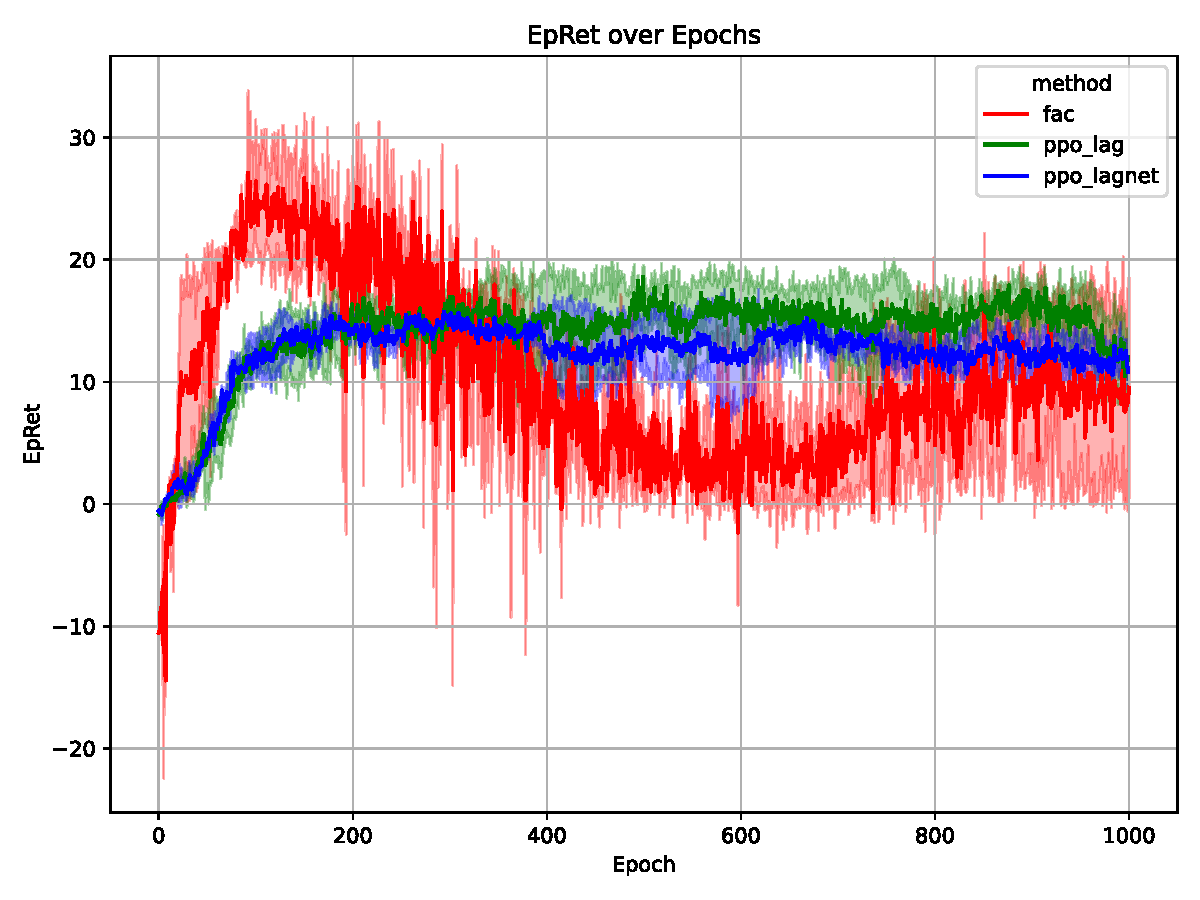
\includegraphics[width=0.65\textwidth]{imgs/chap4/car_goal/return.pdf}
  \caption{Training curves of return over epochs for PPO Lagrangian, Feasible Actor-Critic, and PPO Lagrangian Network on the Car Goal task}
  \label{chap4:fig:car_goal_return}
\end{figure*}

\begin{figure*}[h]
  \centering
  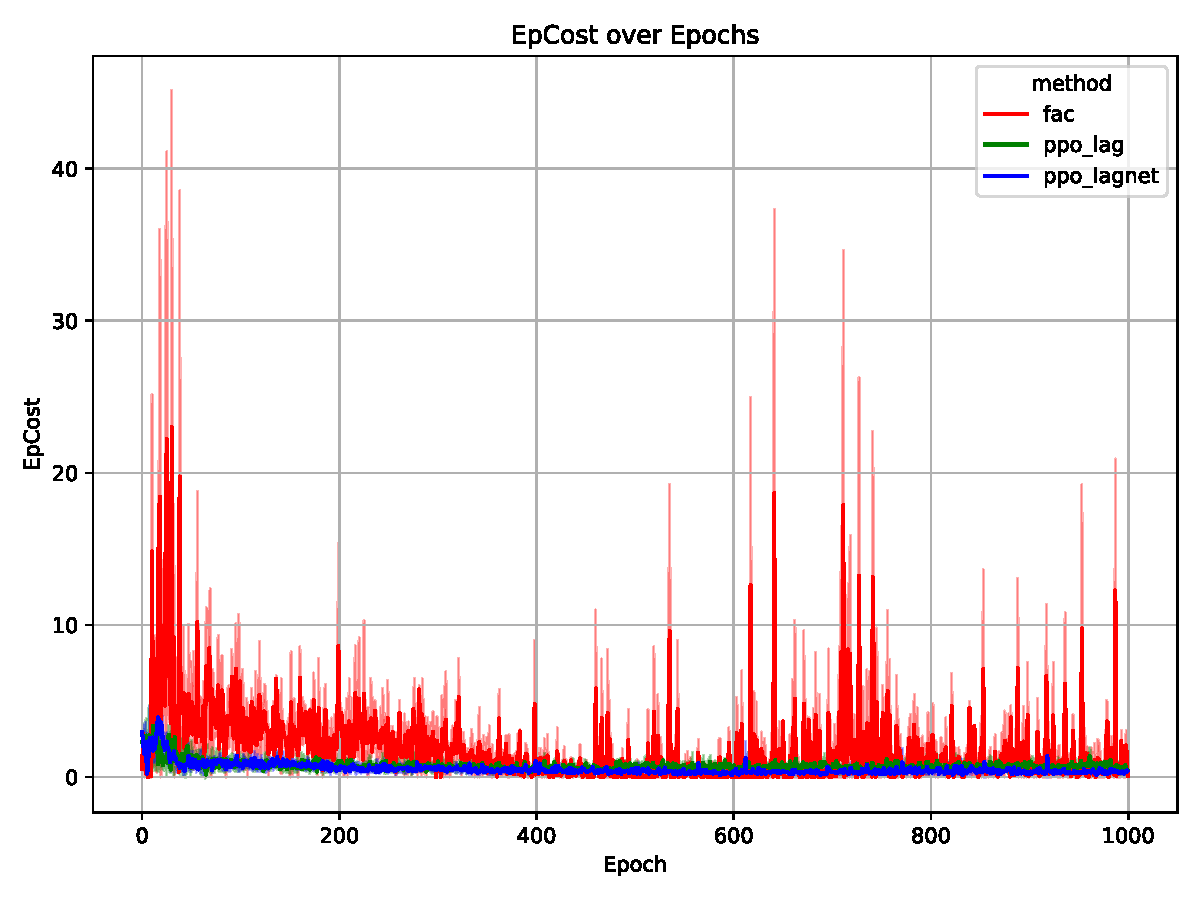
\includegraphics[width=0.65\textwidth]{imgs/chap4/car_goal/cost.pdf}
  \caption{Training curves of cost return over epochs for PPO Lagrangian, Feasible Actor-Critic, and PPO Lagrangian Network on the Car Goal task}
  \label{chap4:fig:car_goal_cost}
\end{figure*}

\clearpage

\begin{figure*}[t]
  \centering
  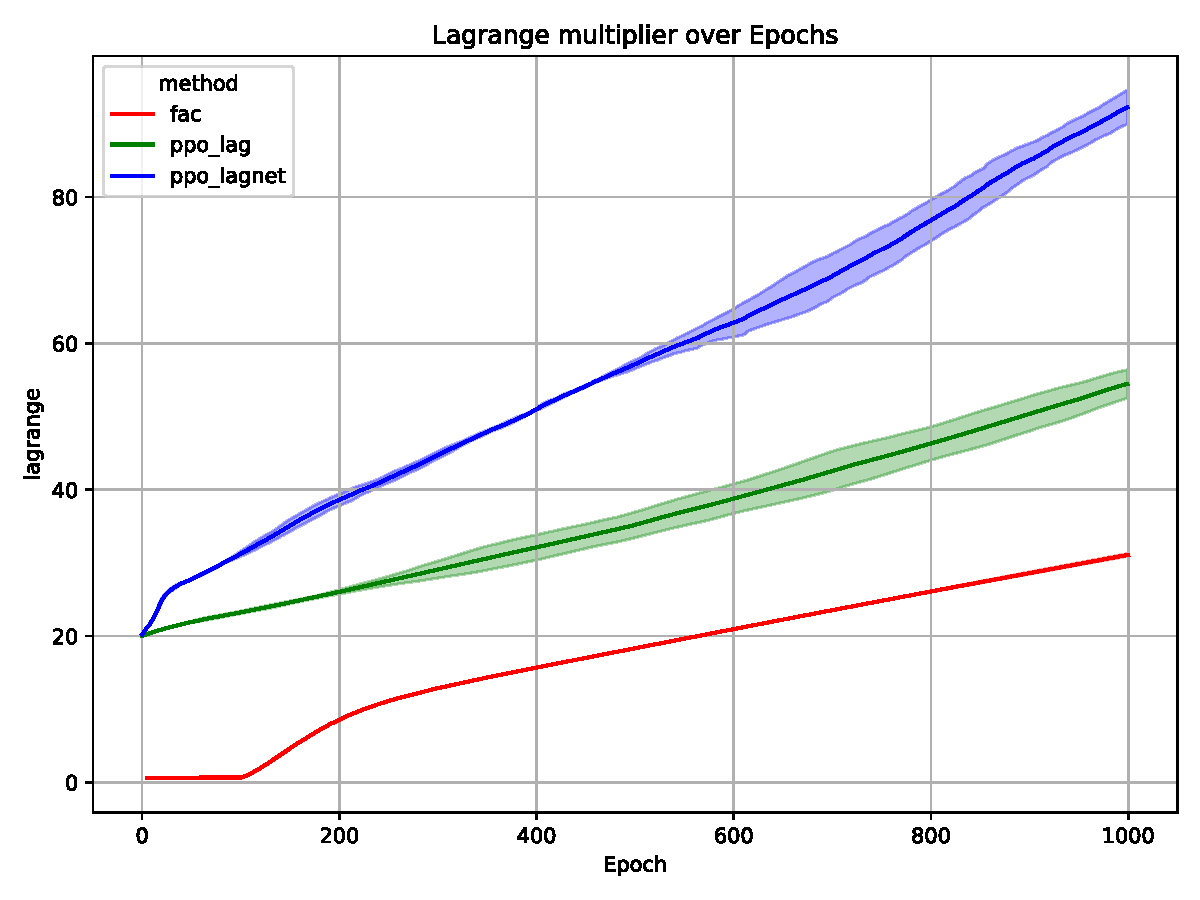
\includegraphics[width=0.65\textwidth]{imgs/chap4/car_goal/lagrange.pdf}
  \caption{Training curves of Lagrange multiplier over epochs for PPO Lagrangian, Feasible Actor-Critic, and PPO Lagrangian Network on the Car Goal task}
  \label{chap4:fig:car_goal_lagrange}
\end{figure*}


\subsection{Car Button}

Unlike the Car Goal task discussed in Section~\ref{chap4:sec5:car_goal}, this task contains more obstacles, which makes policy learning difficult when the cost limit is set to zero (i.e., when any constraint violation is strictly prohibited).
Therefore, in this task, we set the state-wise allowable cost to 0.3, which corresponds to allowing a maximum cumulative cost of 300 per episode (given the episode length is fixed at 1000 steps).
Additionally, since setting the Lagrange multiplier network’s bias to 20 resulted in unstable learning in this task, we initialized it with zero bias in this experiment.
As shown in Fig.~\ref{chap4:fig:car_button_return}, our proposed method demonstrates stable convergence in return.
In contrast, the PPO Lagrangian method (green) shows unstable policy behavior between epochs 300 and 600, followed by performance recovery in the later stages.
For the FAC method, the policy does not improve until around epoch 800, and only starts to receive meaningful rewards after epoch 900.
Looking at Fig.~\ref{chap4:fig:car_button_cost}, we observe that the cost values of FAC begin to increase around the same time its return starts to improve.
These results indicate that FAC needs more training iterations in this task to effectively balance reward acquisition and constraint satisfaction.
Both PPO-based methods (PPO Lagrangian and our proposed method) appear to satisfy the constraints effectively, and in particular, our proposed method maintains stable constraint satisfaction starting from around epoch 100.

\begin{figure*}[h]
  \centering
  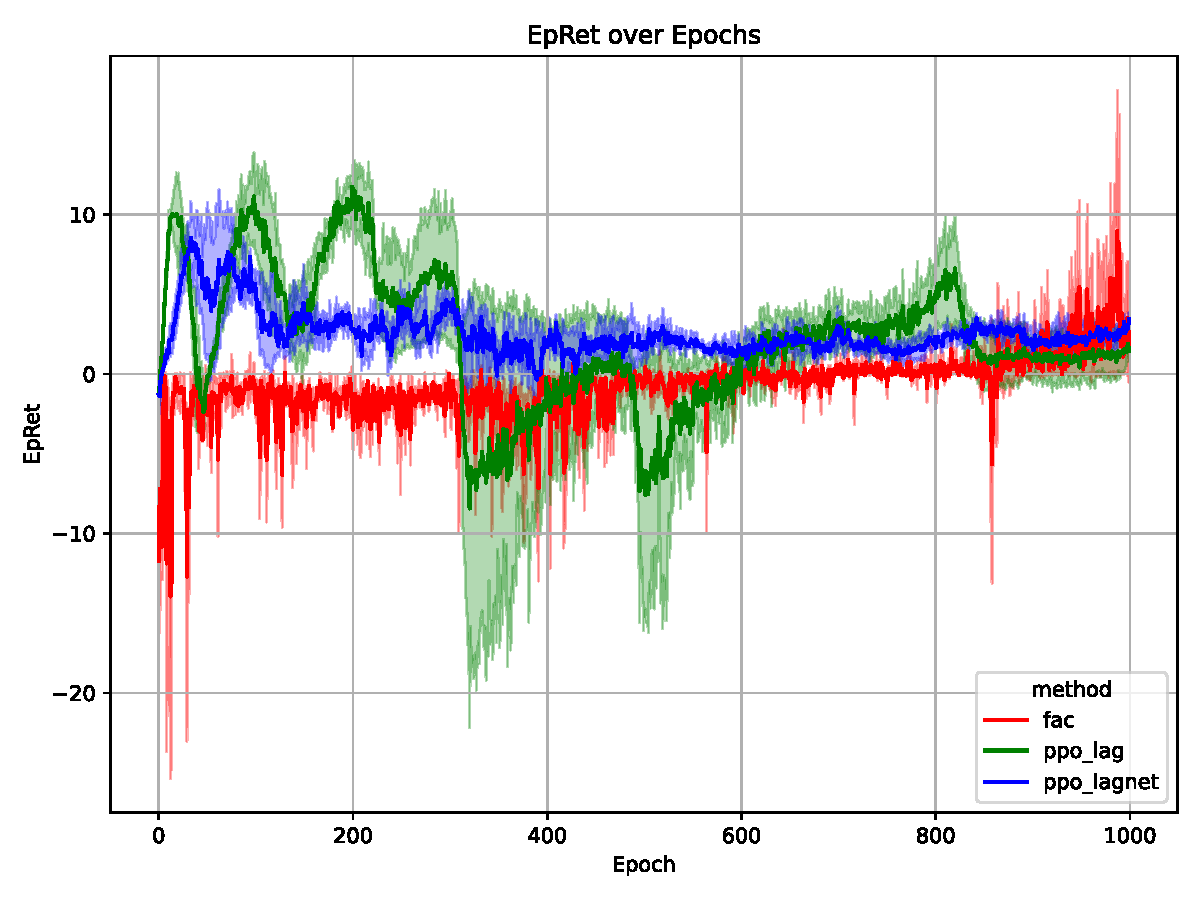
\includegraphics[width=0.7\textwidth]{imgs/chap4/car_button/return.pdf}
  \caption{Training curves of return for PPO Lagrangian, Feasible Actor-Critic, and PPO Lagrangian Network in Car Button task}
  \label{chap4:fig:car_button_return}
\end{figure*}

\begin{figure*}[h]
  \centering
  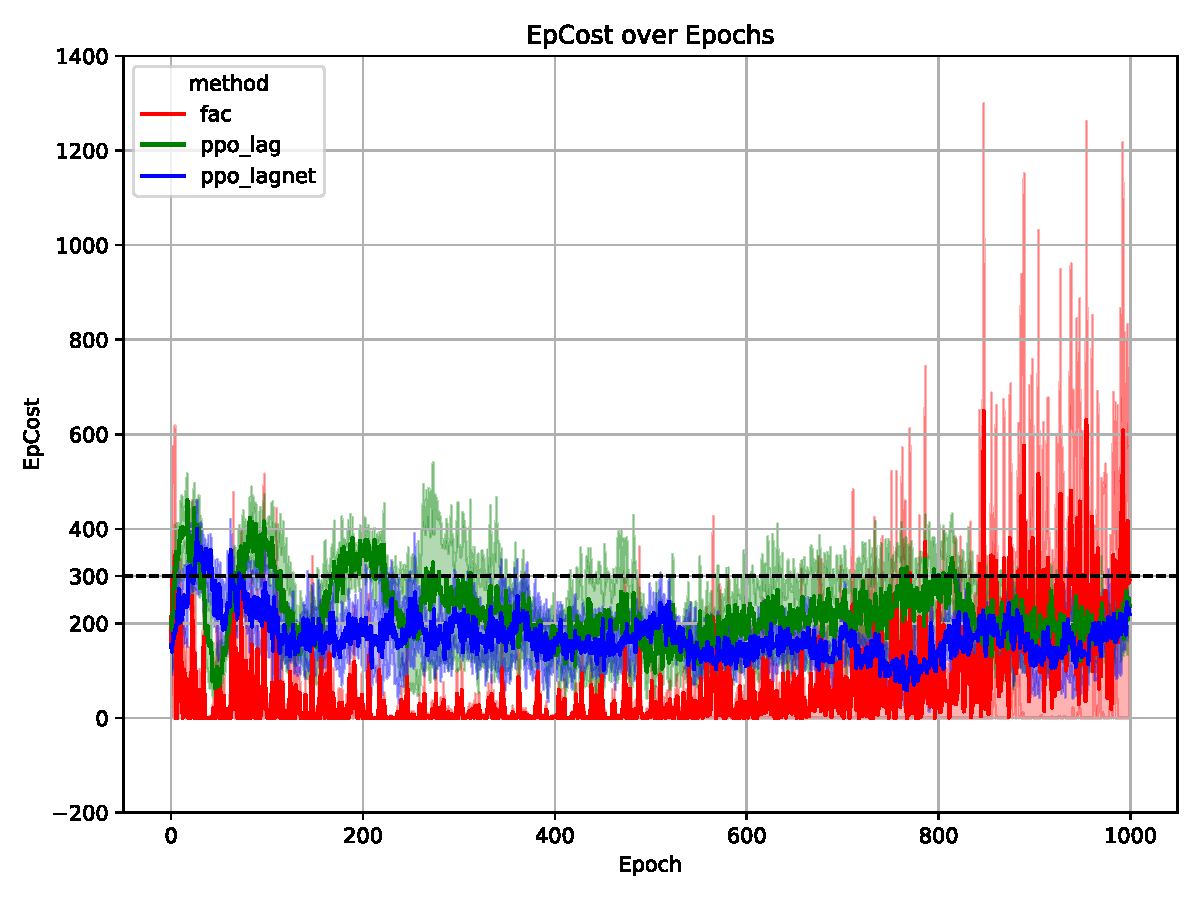
\includegraphics[width=0.7\textwidth]{imgs/chap4/car_button/cost.pdf}
  \caption{Training curves of cost return for PPO Lagrangian, Feasible Actor-Critic, and PPO Lagrangian Network in Car Button task}
  \label{chap4:fig:car_button_cost}
\end{figure*}

\begin{figure*}[h]
  \centering
  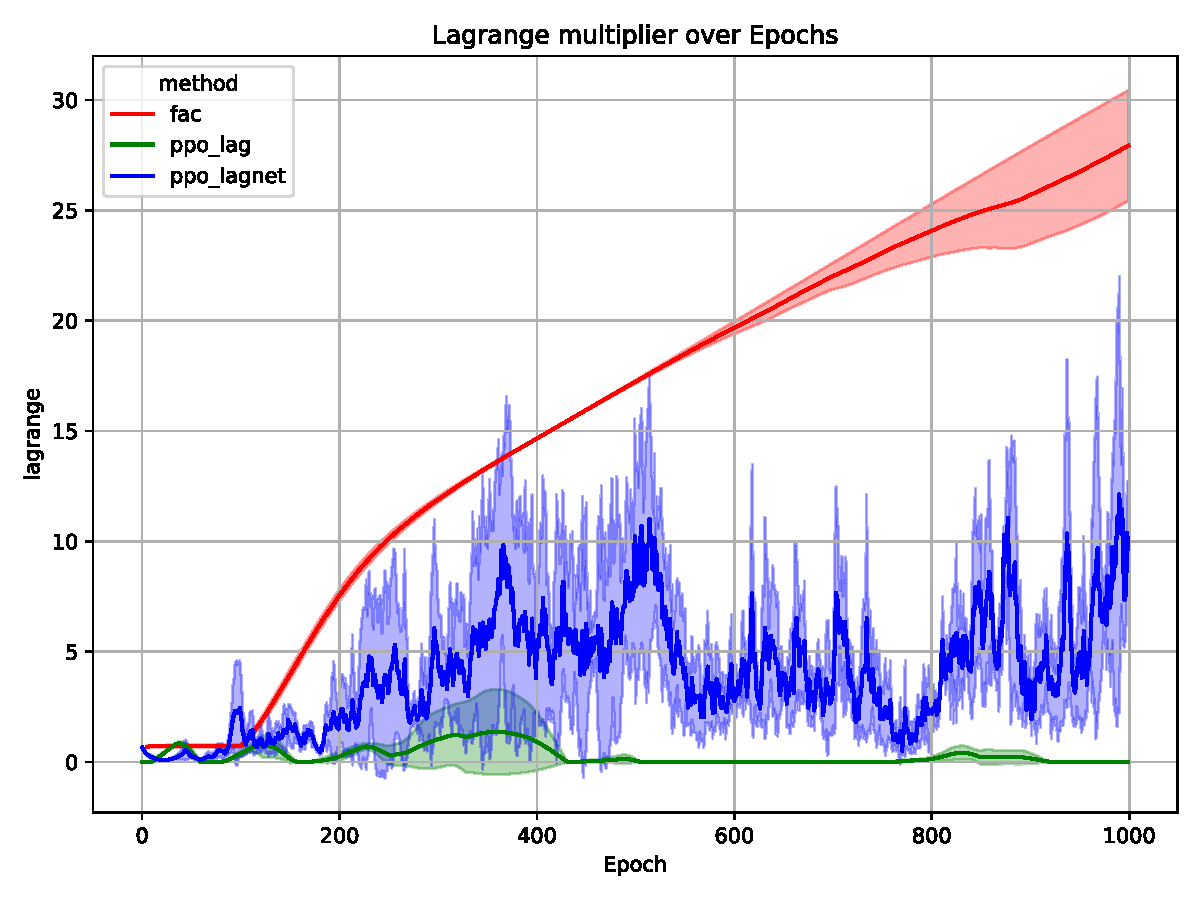
\includegraphics[width=0.7\textwidth]{imgs/chap4/car_button/lagrange.pdf}
  \caption{Training curves of Lagrange multiplier for PPO Lagrangian, Feasible Actor-Critic, and PPO Lagrangian Network in Car Button task}
  \label{chap4:fig:car_button_lagrange}
\end{figure*}

\clearpage

%%%%%%%%%%%%%%%%%%%%%%%%%%%%%%%%
\section{Evaluation Lagrange Multiplier Network}
%%%%%%%%%%%%%%%%%%%%%%%%%%%%%%%%

In this section, we evaluate the performance of the Lagrange multiplier network trained in the Point Goal task.
We utilize the trained Lagrange multiplier network at test time, thereby enabling the assessment of whether the current state is potentially unsafe.
As illustrated in Fig.~\ref{chap4:fig:lagrange_test1} and Fig.~\ref{chap4:fig:lagrange_test2}, the trained Lagrange multiplier network outputs (displayed in the top-right corner of each figure) near-zero or low values when the agent is in a safe state, meaning there are no nearby obstacles or the agent is not moving toward hazardous regions.
As the agent approaches obstacles, the output of the network gradually increases, indicating a higher level of potential risk.
These results demonstrate that the Lagrange multiplier network has successfully learned to assign appropriate penalties based on the agent’s proximity to unsafe areas.
Therefore, it can be effectively used at test time to assess the safety of a given state.

\begin{figure*}[h]
  \centering
  \subfloat[Step 2170]{%
    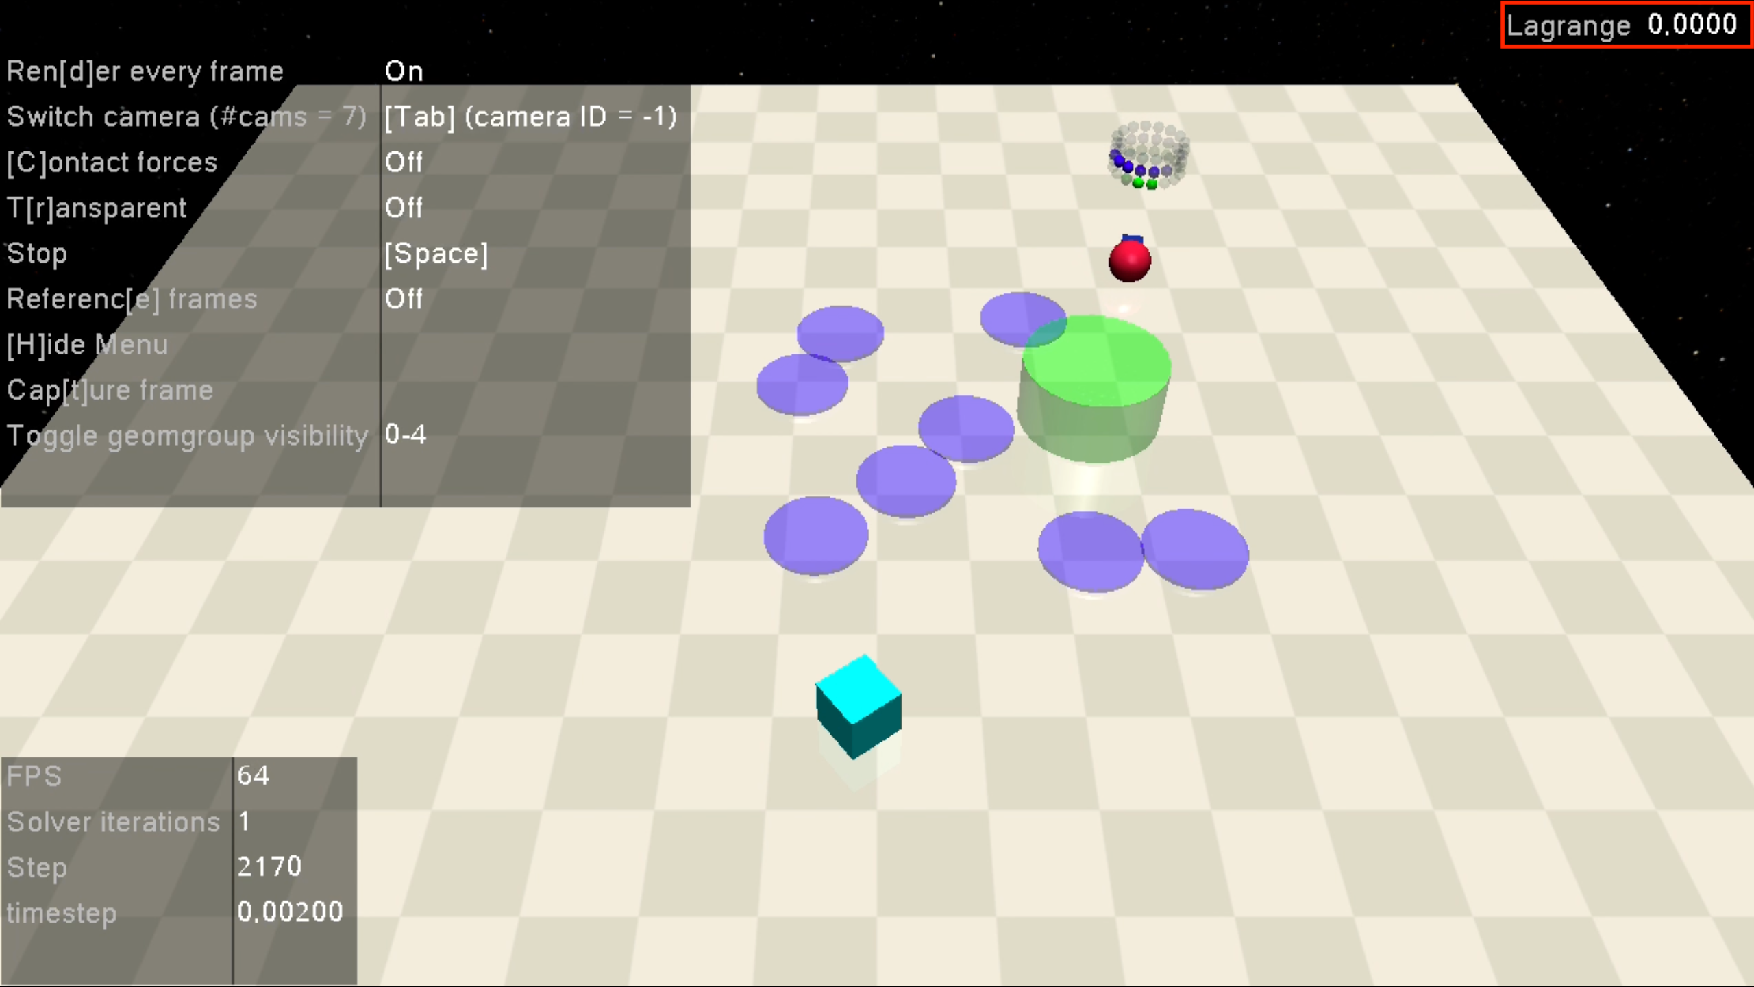
\includegraphics[width=0.7\textwidth]{imgs/chap4/lagrange/test1/0.pdf}
  }

  \vspace{0.2em}

  \subfloat[Step 2450]{%
    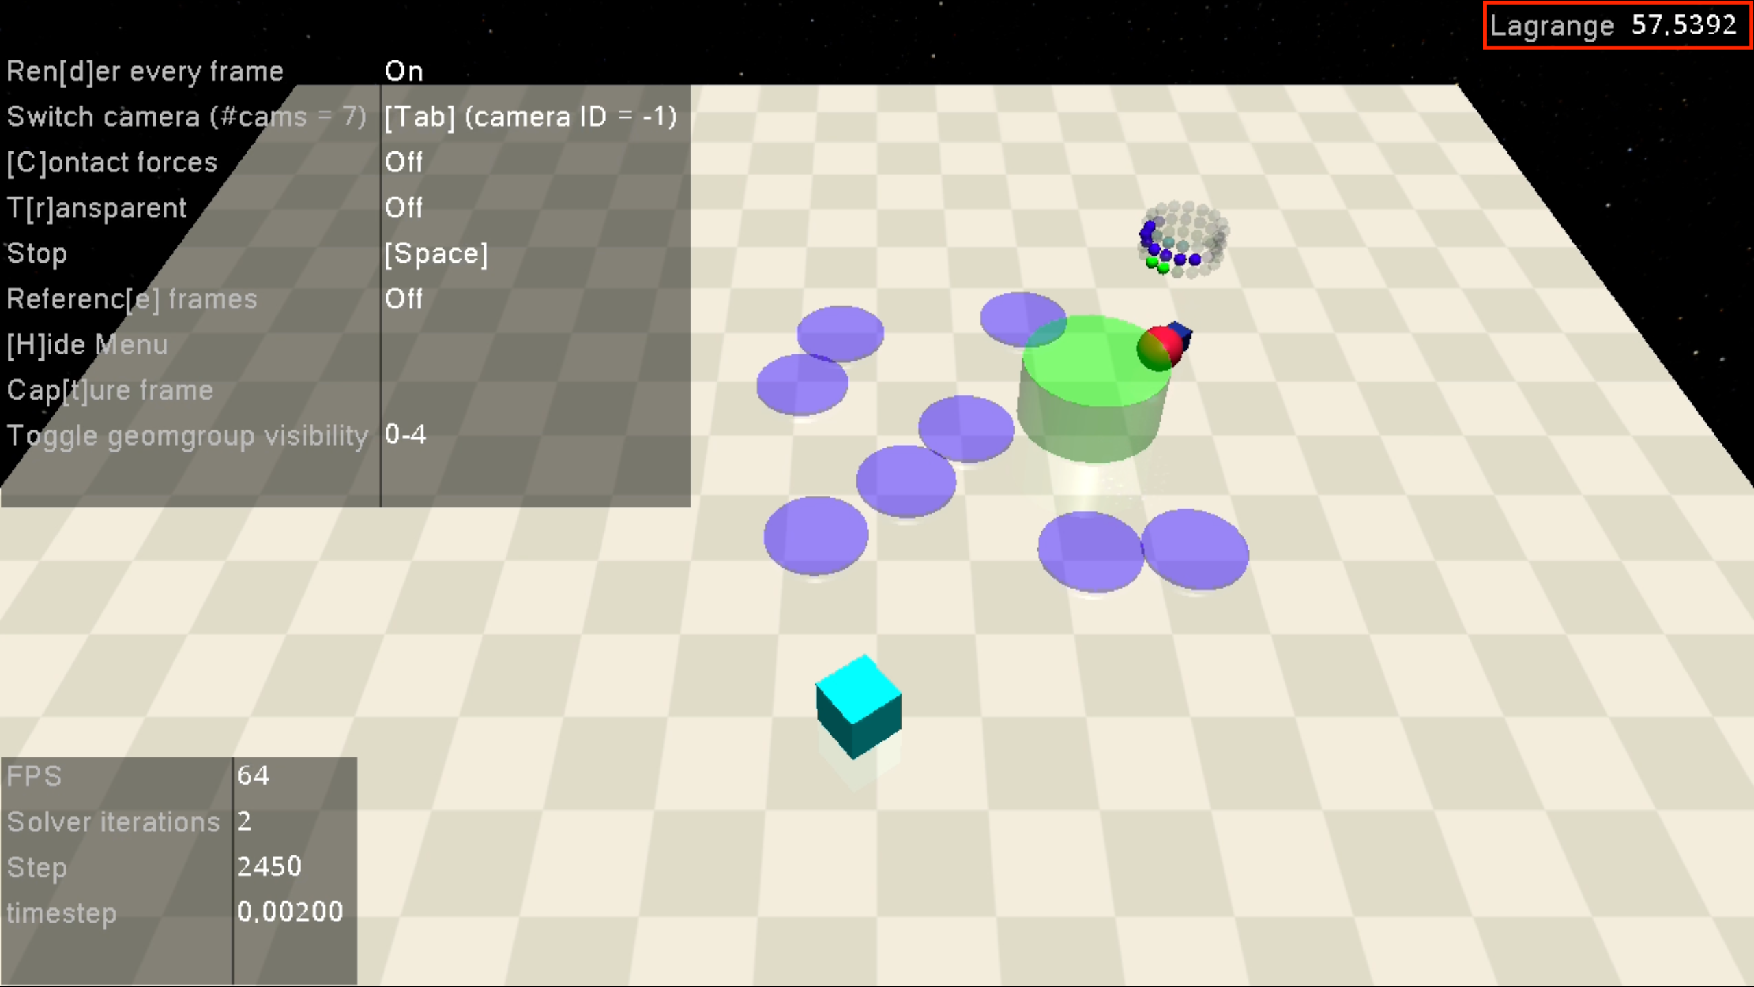
\includegraphics[width=0.7\textwidth]{imgs/chap4/lagrange/test1/50.pdf}
  }

  \vspace{0.2em}

  \subfloat[Step 2670]{%
    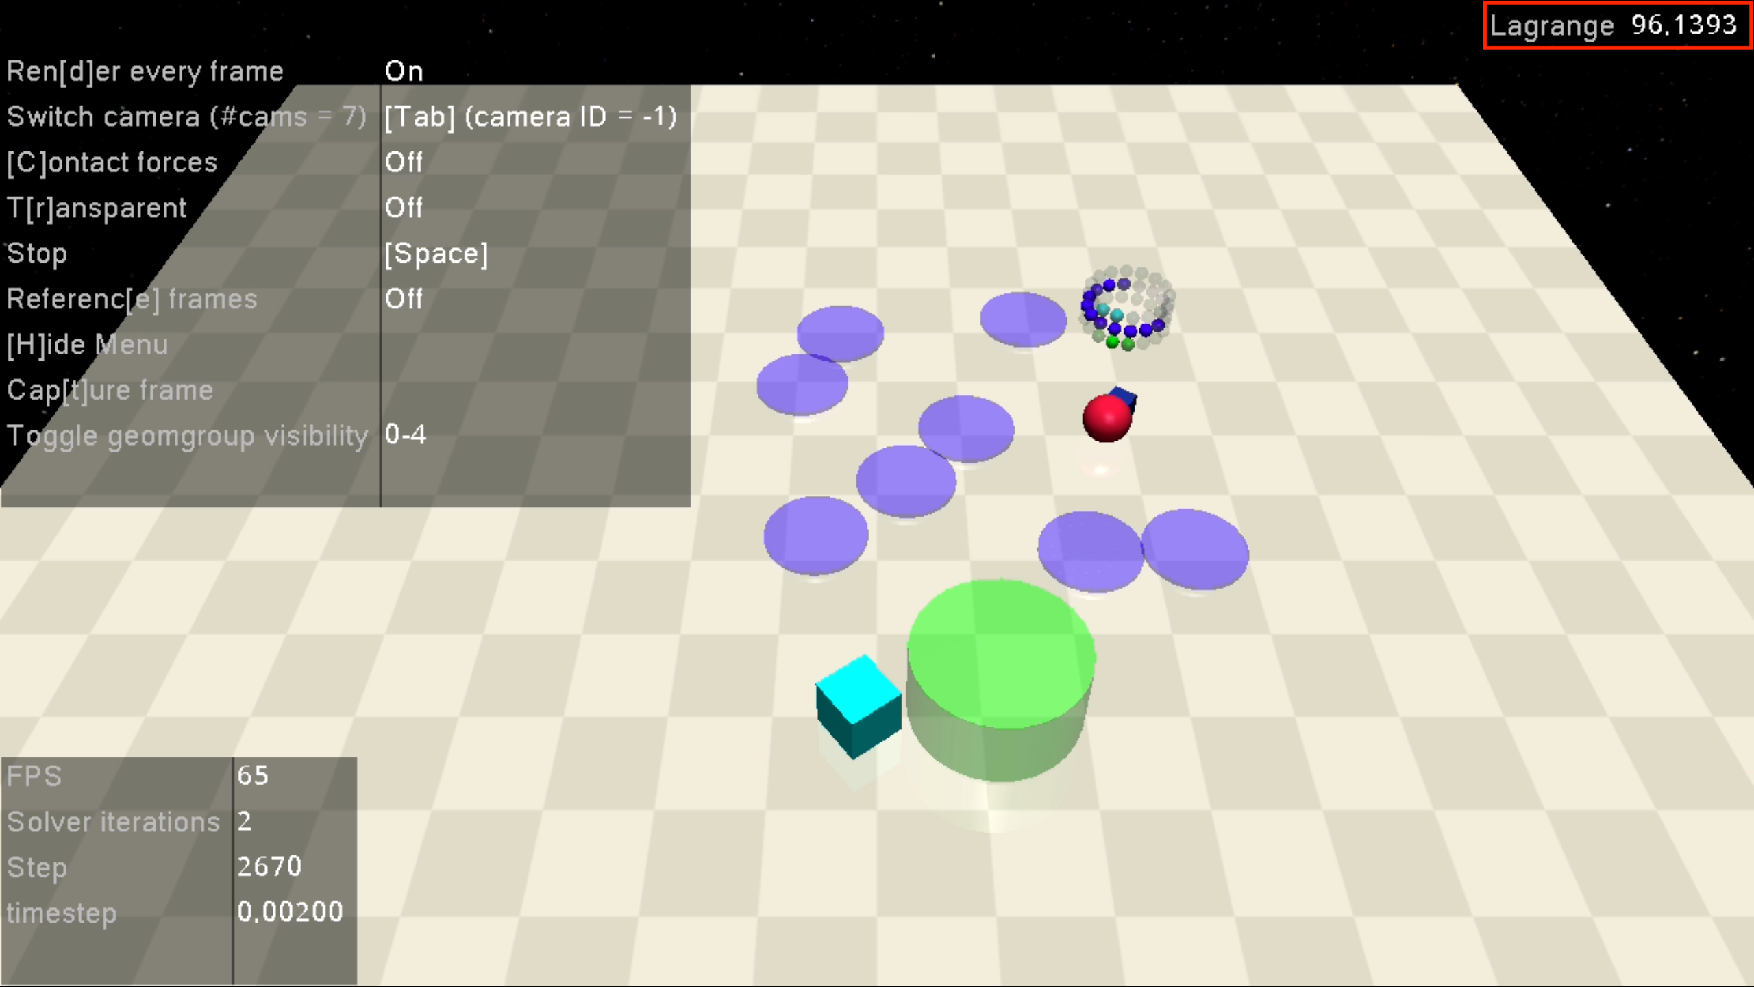
\includegraphics[width=0.7\textwidth]{imgs/chap4/lagrange/test1/90.pdf}
  }

  \caption{Visualization of the Lagrange multiplier network output at different steps in the test scenario 1}
  \label{chap4:fig:lagrange_test1}
\end{figure*}

\begin{figure*}[h]
  \centering
  \subfloat[Step 4640]{%
    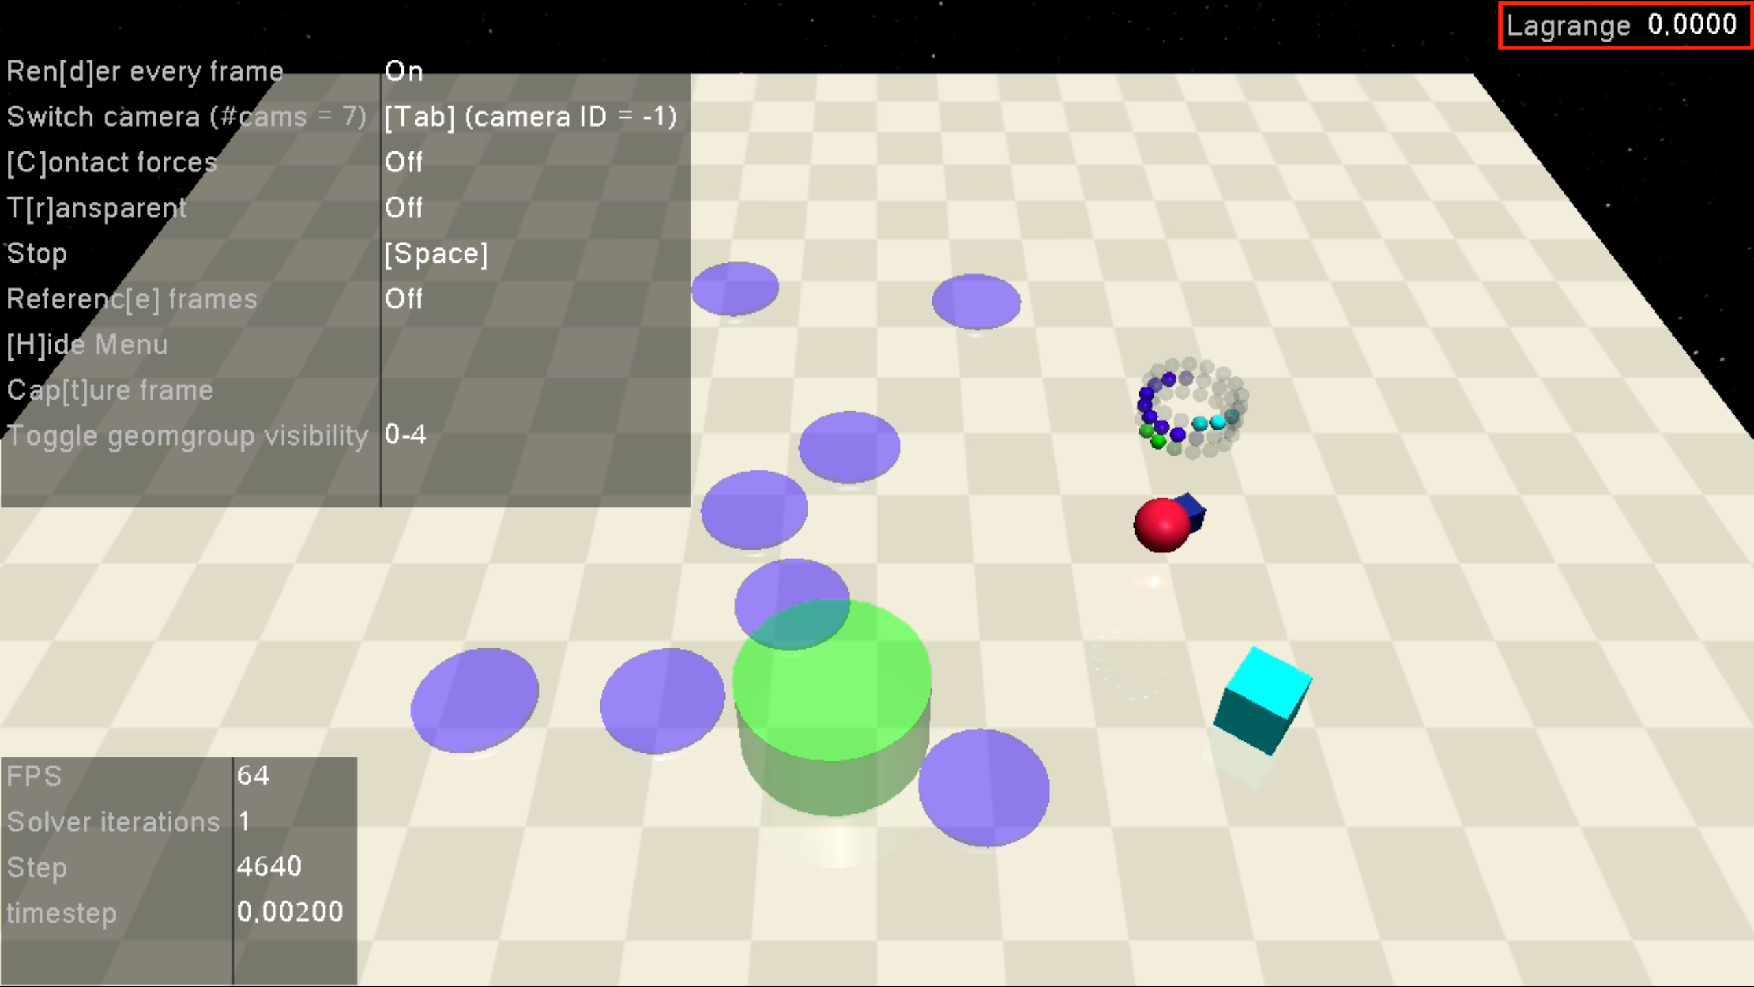
\includegraphics[width=0.7\textwidth]{imgs/chap4/lagrange/test2/0.pdf}
  }

  \vspace{0.2em}

  \subfloat[Step 4850]{%
    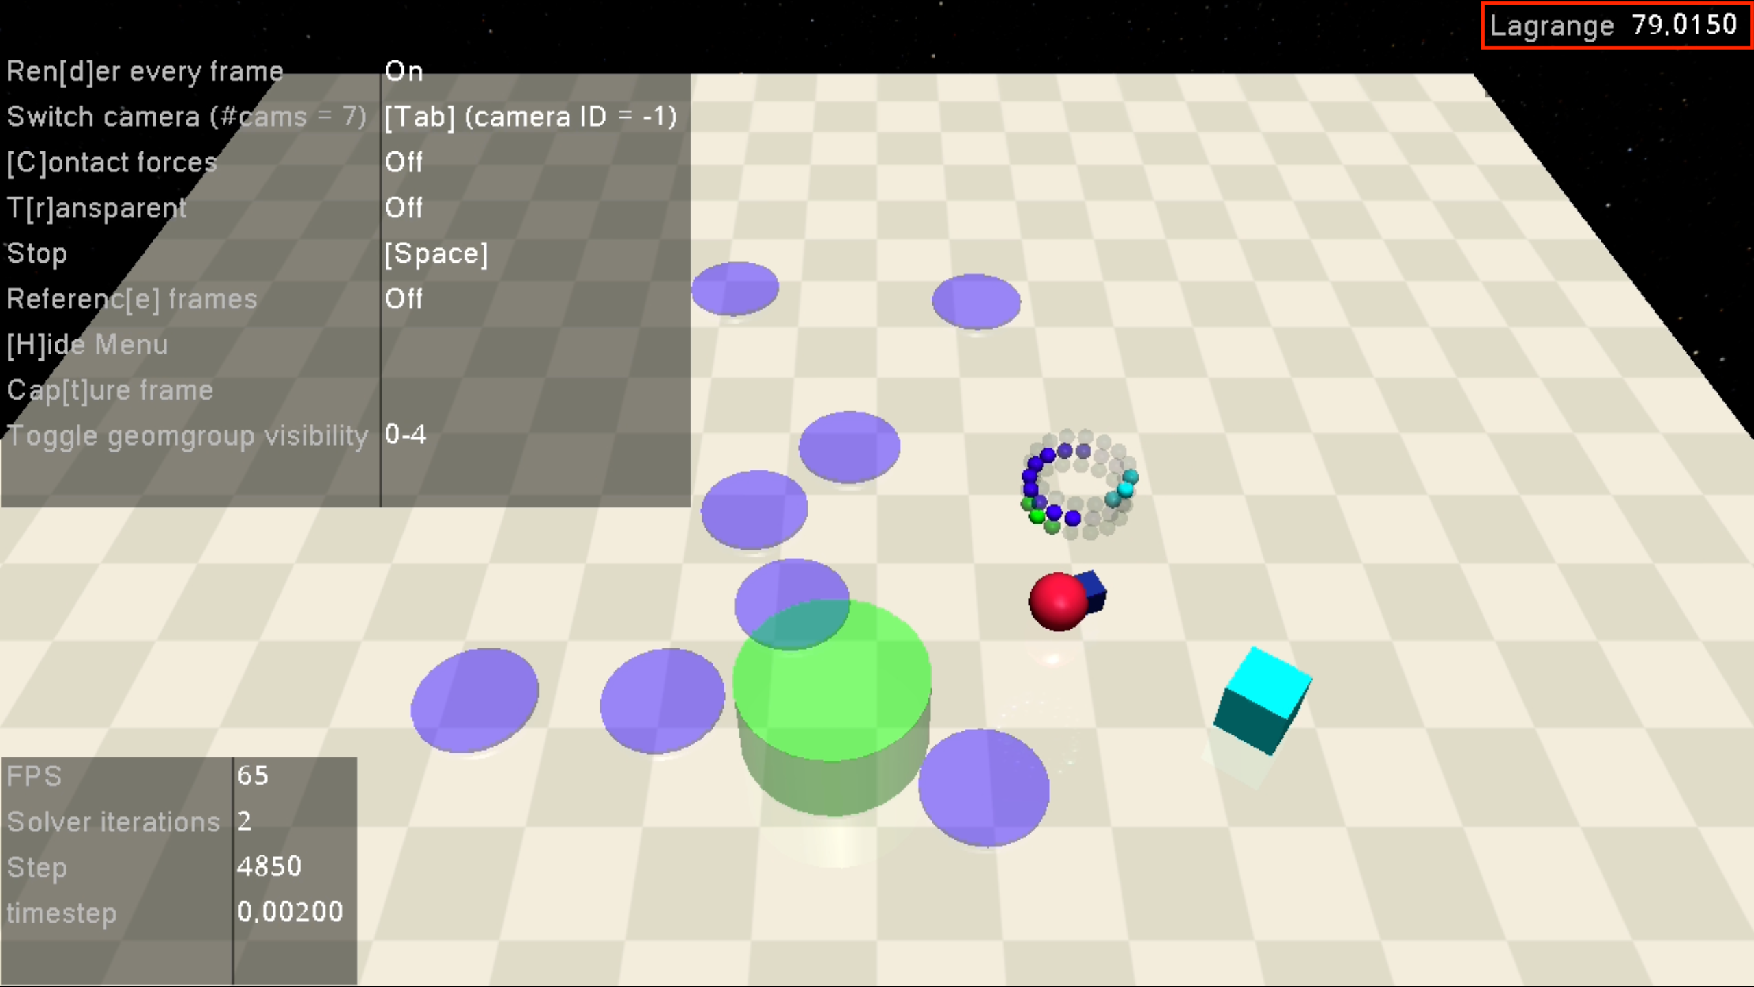
\includegraphics[width=0.7\textwidth]{imgs/chap4/lagrange/test2/80.pdf}
  }

  \caption{Visualization of the Lagrange multiplier network output at different steps in the test scenario 2}
  \label{chap4:fig:lagrange_test2}
\end{figure*}